\documentclass{beamer}

\usepackage{amsmath}
\usepackage{amssymb}
\usepackage{graphics}

\begin{document}

\section*{Checking for Normality}
\begin{frame}
\frametitle{Normal Probability Plots}
\Large
\begin{itemize}
\item A normal distribution is often a reasonable model for the data. Without inspecting the data, however, it is risky to assume a normal distribution. 

\item There are a number of graphs that can be used to check the deviations of the data from the normal distribution. 

\end{itemize}

\end{frame}
%-------------------------------------------------------------------------- %
\begin{frame}
\frametitle{Normal Probability Plots}
\Large
\begin{itemize}
\item A histogram is an example of a graph that can be used to check normality. \item Here, the histogram should reveal a bell shaped curve. 
\end{itemize}
\begin{figure}
\centering
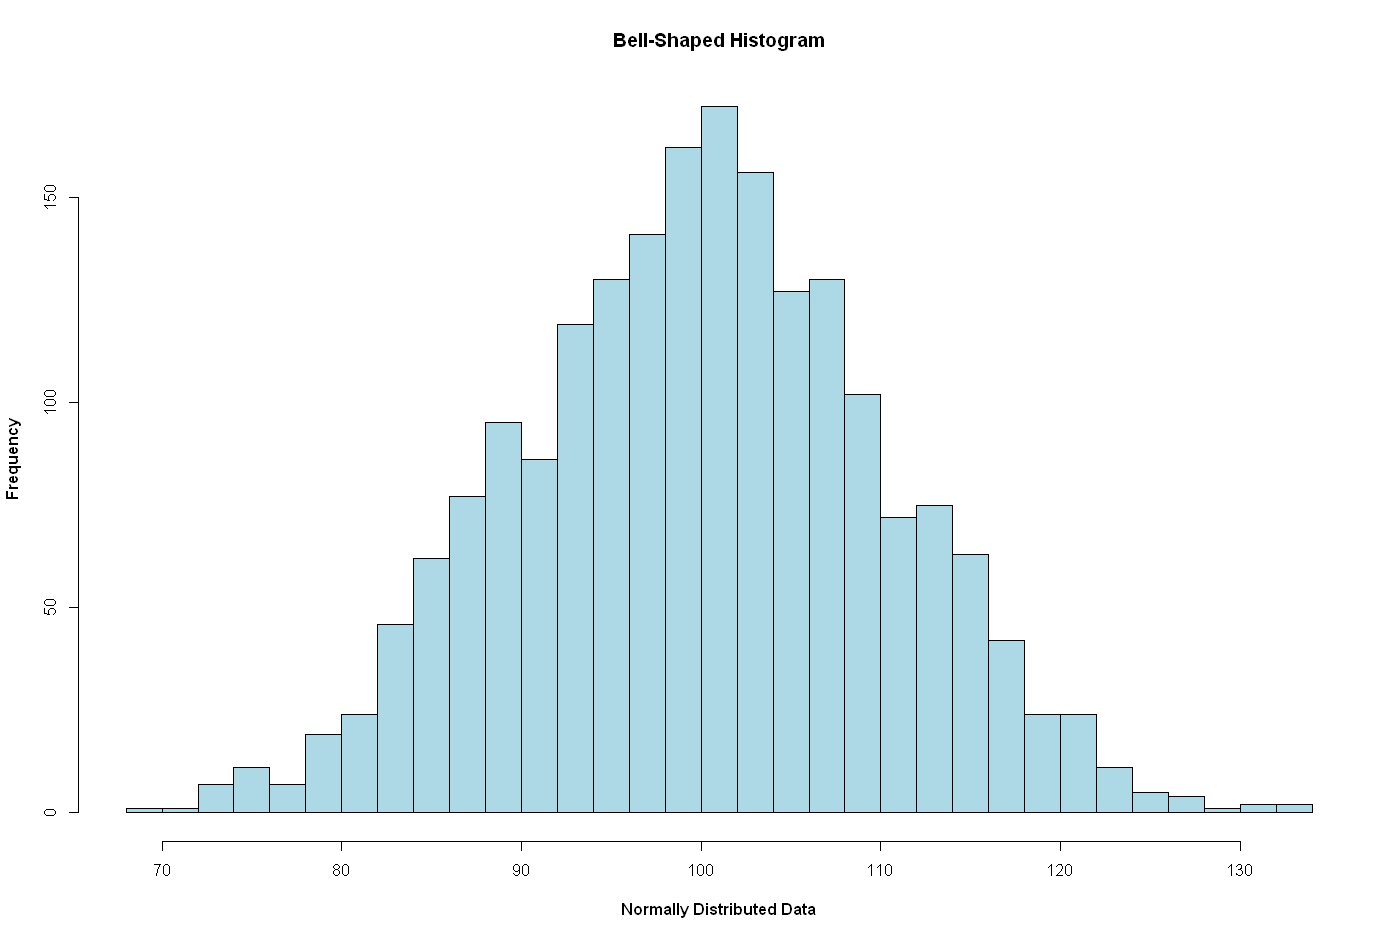
\includegraphics[width=0.7\linewidth]{./LargeXNormHist}
\label{fig:LargeXNormHist}
\end{figure}

\end{frame}
%-------------------------------------------------------------------------- %
\begin{frame}
\frametitle{Normal Probability Plots}
\Large

\begin{figure}
\centering
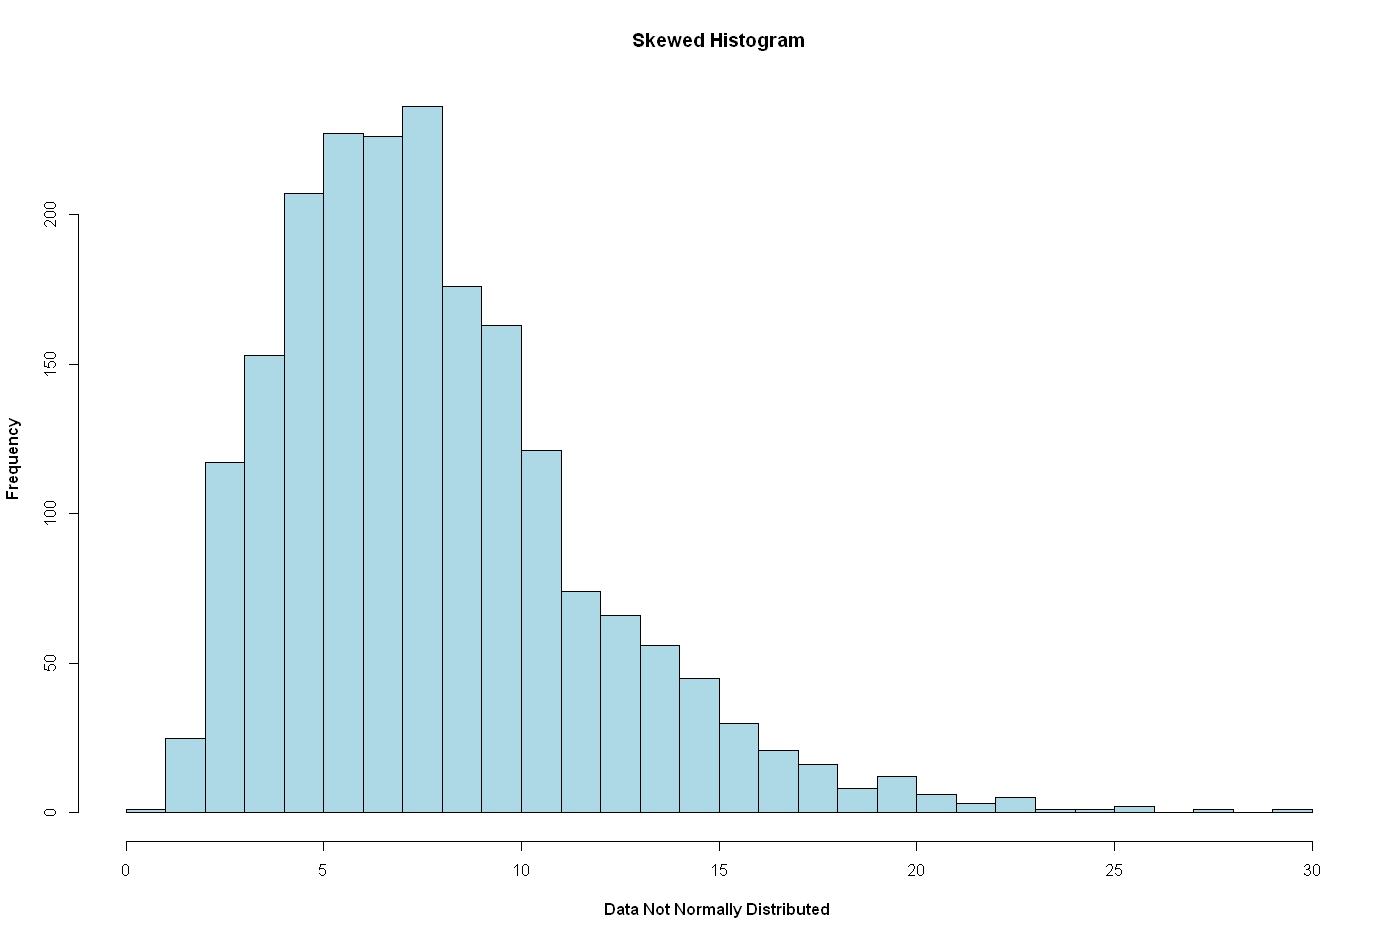
\includegraphics[width=0.7\linewidth]{./LargeXNotNormHist}
\label{fig:LargeXNotNormHist}
\end{figure}

\end{frame}
%------------------------------------------------- %
\begin{frame}
\frametitle{Normal Probability Plots}
\Large
\begin{itemize}

\item The most useful tool for assessing normality is a \textit{\textbf{quantile -quantile}} or \textbf{Q-Q} plot. \item This is a scatterplot with the quantiles of the scores on the horizontal axis and the equivalent values expected when assuming the normal distribution, on the vertical axis. 
\end{itemize}
\end{frame}
%------------------------------------------------- %
\begin{frame}
\frametitle{Normal Probability Plots}
\Large
\begin{itemize}
\item The steps in constructing a QQ plot are as follows: First, we sort the data from smallest to largest. 
\item A plot of these scores against the expected normal scores should reveal a straight line. \item The expected normal scores are calculated by taking the z-scores  where I is the rank in increasing order.
\end{itemize}
\end{frame}
%------------------------------------------------- %
\begin{frame}
\frametitle{Normal Probability Plots}
\Large
\begin{itemize}

\item Curvature of the points indicates departures of normality. This plot is also useful for detecting outliers. The outliers appear as points that are far away from the overall pattern op points
\end{itemize}
\end{frame}
%------------------------------------------------- %
\begin{frame}
\frametitle{Normal Probability Plots}

\end{frame}
\end{document}